% SmO2 Control: Funktionsweise, Formeln und Beispielrechnungen.
%
% Alle Zahlen kommen aus numbers.tex, das figures.py aus einer echten Einheit
% erzeugt. Nichts ist von Hand eingetragen; wer die Datei wechselt, bekommt ein
% Dokument mit den Zahlen dieser Datei.
%
% Bauen:  ./build.sh     (latexmk, siehe dort)

\documentclass[11pt,a4paper]{article}

\usepackage[T1]{fontenc}
\usepackage[utf8]{inputenc}
\usepackage[ngerman]{babel}
\usepackage{lmodern}
\usepackage{microtype}
\usepackage[a4paper,margin=25mm,top=22mm,bottom=25mm]{geometry}
\usepackage{amsmath,amssymb}
\usepackage{graphicx}
\usepackage{booktabs}
\usepackage{tabularx}
\usepackage{caption}
\usepackage{float}
\usepackage{placeins}
\usepackage{enumitem}
\usepackage{xcolor}
\usepackage[autostyle]{csquotes}
\usepackage[locale=DE,per-mode=symbol,separate-uncertainty=true,
            range-phrase={ bis },range-units=single]{siunitx}
\usepackage[hidelinks,pdftitle={SmO2 Control: Kinetik, Zustaende, Metriken, Prognose},
            pdfauthor={SmO2 Control}]{hyperref}
\usepackage[ngerman,nameinlink,noabbrev]{cleveref}

% generated by figures.py, do not edit
\newcommand{\nFile}{i182958466.fit}
\newcommand{\nN}{4449}
\newcommand{\nHoltRawA}{47.6}
\newcommand{\nHoltRawB}{47.6}
\newcommand{\nHoltRawC}{47.3}
\newcommand{\nHoltMed}{47.6}
\newcommand{\nHoltDt}{1.0}
\newcommand{\nHoltLprev}{47.351}
\newcommand{\nHoltTprev}{-0.1116}
\newcommand{\nHoltFc}{47.240}
\newcommand{\nHoltL}{47.348}
\newcommand{\nHoltSlope}{-0.0035}
\newcommand{\nHoltT}{-0.0953}
\newcommand{\nRegN}{7}
\newcommand{\nRegSy}{341.139}
\newcommand{\nRegSxy}{1019.904}
\newcommand{\nRegSx}{21}
\newcommand{\nRegSxx}{91}
\newcommand{\nRegPerSample}{-0.1255}
\newcommand{\nRegSpan}{6}
\newcommand{\nRegSlope}{-0.1255}
\newcommand{\nRegSlopeSixty}{-0.0335}
\newcommand{\nRegT}{120}
\newcommand{\nRegRows}{0 & 49.309 \\
1 & 48.999 \\
2 & 48.764 \\
3 & 48.562 \\
4 & 48.418 \\
5 & 48.501 \\
6 & 48.586 \\}
\newcommand{\nHoltOutBand}{53}
\newcommand{\nHoltOutFifteen}{22}
\newcommand{\nPlateauN}{290}
\newcommand{\nFcLap}{Runde 02}
\newcommand{\nFcT}{40}
\newcommand{\nFcLevel}{51.45}
\newcommand{\nFcTrend}{-0.359}
\newcommand{\nFcPred}{46.06}
\newcommand{\nFcActual}{47.24}
\newcommand{\nFcErr}{1.17}
\newcommand{\nFcRmseAll}{6.93}
\newcommand{\nFcRmseNaive}{5.11}
\newcommand{\nSciStart}{66.0}
\newcommand{\nSciEnd}{46.4}
\newcommand{\nSciDur}{359}
\newcommand{\nSciDrop}{19.7}
\newcommand{\nSciRatio}{0.70}
\newcommand{\nSciRate}{-0.055}
\newcommand{\nStepsRows}{1 & 359 & 66.0 & 46.4 & 19.7 & 0.70 & -0.055 & 78 \\
2 & 360 & 75.8 & 46.3 & 29.6 & 0.61 & -0.082 & 58 \\
3 & 359 & 71.3 & 38.8 & 32.5 & 0.54 & -0.091 & 47 \\
4 & 359 & 76.2 & 39.4 & 36.8 & 0.52 & -0.103 & 68 \\
5 & 360 & 78.9 & 35.3 & 43.6 & 0.45 & -0.121 & 51 \\
6 & 360 & 79.8 & 37.7 & 42.1 & 0.47 & -0.117 & 47 \\}
\newcommand{\nSynOneSteady}{58}
\newcommand{\nSynOneOnkin}{34}
\newcommand{\nSynThreeSteady}{7}
\newcommand{\nSynThreeOnkin}{42}
\newcommand{\nFcRmseOnset}{10.61}
\newcommand{\nFcRmseRecover}{6.78}
\newcommand{\nFcRmseHolding}{5.44}
\newcommand{\nFcRmseDrifting}{6.65}
\newcommand{\nFcRmseFalling}{7.58}
\newcommand{\nDwellOne}{22}
\newcommand{\nRunsOne}{152}
\newcommand{\nDwellTwo}{21}
\newcommand{\nRunsTwo}{151}
\newcommand{\nDwellThree}{13}
\newcommand{\nRunsThree}{143}
\newcommand{\nDwellFour}{8}
\newcommand{\nRunsFour}{135}


\captionsetup{font=small,labelfont=bf,width=0.92\textwidth}
\setlist{nosep}

% Zustandsfarben, die Druckvarianten aus figures.py
\definecolor{recover}{HTML}{0B5CB5}
\definecolor{holding}{HTML}{1E7A34}
\definecolor{drifting}{HTML}{B08900}
\definecolor{falling}{HTML}{B71C1C}
\definecolor{onset}{HTML}{EF6C00}
\newcommand{\st}[2]{\textcolor{#1}{\textbf{#2}}}
\newcommand{\RECOVER}{\st{recover}{RECOVER}}
\newcommand{\HOLDING}{\st{holding}{HOLDING}}
\newcommand{\DRIFTING}{\st{drifting}{DRIFTING}}
\newcommand{\FALLING}{\st{falling}{FALLING}}
\newcommand{\ONSET}{\st{onset}{ONSET}}

\newcommand{\smo}{SmO\textsubscript{2}}
\newcommand{\pers}{\si{\percent\per\second}}
\newcommand{\permin}{\si{\percent\per\minute}}

\title{\textbf{SmO\textsubscript{2} Control}\\[4pt]
  \large Echtzeit-Kinetikanalyse der Muskeloxygenierung auf einer Sportuhr:\\
  Modell, Zustände, Metriken und Prognose}
\author{Funktionsbeschreibung mit Formeln und Beispielrechnungen\\
  \small aus der aufgezeichneten Einheit \texttt{\nFile} (\num{\nN} Messwerte)}
\date{\today}

\begin{document}
\maketitle

\begin{abstract}
\noindent
SmO\textsubscript{2} Control ist ein Connect-IQ-Datenfeld, das einen
Moxy-Muskeloxygenierungssensor über ANT+ liest und aus dem Signal in Echtzeit
eine Antwort auf eine Frage ableitet: Befindet sich die Muskulatur in einem
Steady State, oder sinkt die Sättigung weiter? Dieses Dokument beschreibt das
Modell vollständig: den Medianvorfilter, die Holt-Glättung, die
Regressionssteigung über ein 60-Sekunden-Fenster, die fünf Zustände mit
Hysterese und Verweildauer, die Behandlung des On-Transienten, die
abgeleiteten Metriken einschließlich des Control Index sowie die
Kurzzeitprognose. Jede Formel wird an Zahlen aus einer echten Einheit
nachgerechnet, und jede Abbildung stammt aus derselben Berechnung, die auch die
Uhr ausführt. Ein Ergebnis fällt dabei gegen das Modell aus und wird als
solches berichtet: Die 15-Sekunden-Prognose ist auf dieser Einheit schlechter
als die Annahme, der Wert bleibe, wo er ist.
\end{abstract}

% Sections only: with subsections the list spills its last line onto a page
% of its own.
\setcounter{tocdepth}{1}
\tableofcontents
\clearpage

% ---------------------------------------------------------------------------
\section{Fragestellung und Signal}

Nahinfrarotspektroskopie (NIRS) misst die Sauerstoffsättigung des Hämoglobins
im Muskelgewebe unter dem Sensor, \smo{} in Prozent. Der Absolutwert ist
zwischen Einheiten kaum vergleichbar: Er hängt von der Sensorstelle, der
Fettschichtdicke, dem Anpressdruck des Gurts und der Tagesform ab. Innerhalb
einer Einheit ist er dagegen sehr informativ, und zwar über seine
\emph{Kinetik}: wie schnell die Sättigung zu Beginn einer Belastung fällt, ob
sie ein Plateau erreicht, und wie schnell sie sich erholt.

Physiologisch entspricht ein Plateau einem Gleichgewicht von Sauerstoffangebot
und -verbrauch, also einem Steady State. Sinkt die Sättigung bei konstanter
äußerer Last weiter, besteht dieses Gleichgewicht nicht. Die Frage des
Datenfelds ist damit eine Frage nach der \emph{Steigung} der Kurve, nicht nach
ihrem Wert, und daraus folgt die wichtigste Eigenschaft des Systems: Es braucht
keine Kalibrierung. Eine Steigung in \pers{} bedeutet auf jedem Niveau
dasselbe.

Der Moxy liefert etwa einen Messwert pro Sekunde. Das Signal ist verrauscht,
und sein charakteristischer Fehler ist nicht das Rauschen, sondern der
einzelne Ausreißer: eine Lesung, die um zwanzig Punkte springt und sofort
zurückkommt, oder eine Sekunde, die als ungültig gemeldet wird.
\Cref{fig:signal} zeigt ein Arbeitsintervall der Referenzeinheit mit Rohwerten,
geglättetem Level und den daraus bestimmten Zuständen.

\begin{figure}[H]
  \centering
  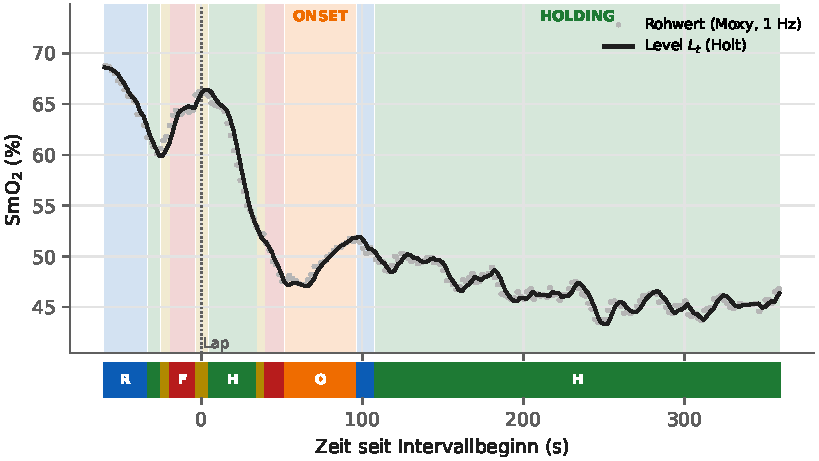
\includegraphics[width=\textwidth]{figures/signal.pdf}
  \caption{Ein Arbeitsintervall (\SI{\nSciDur}{\second}) mit den 60 Sekunden davor.
    Graue Punkte: Rohwerte des Sensors. Schwarze Linie: geglätteter Level
    $L_t$. Die Bänder und der Streifen darunter zeigen den vom Modell
    bestimmten Zustand; der Buchstabe im Streifen ist der Anfangsbuchstabe des
    Zustands. Das Intervall beginnt mit einem steilen Abfall (\ONSET{}) und
    erreicht danach ein Plateau (\HOLDING{}), was es als nachhaltige Belastung
    ausweist.}
  \label{fig:signal}
\end{figure}

% ---------------------------------------------------------------------------
\section{Signalverarbeitung}

Das Modell besteht aus drei Stufen, die nacheinander auf jeden Messwert
angewendet werden: ein Medianvorfilter, eine Holt-Glättung für den Level, und
eine lineare Regression über ein festes Zeitfenster für die Steigung. Die
Klassifikation arbeitet ausschließlich auf der Regressionssteigung.
\Cref{tab:symbols} listet die Symbole.

\begin{table}[H]
  \centering\small
  \caption{Symbole und Standardwerte.}
  \label{tab:symbols}
  \begin{tabular}{@{}llc@{}}
    \toprule
    Symbol & Bedeutung & Standard \\
    \midrule
    $x_t$ & Rohwert des Sensors zum Zeitpunkt $t$ & \\
    $v_t$ & Median der letzten drei Rohwerte & $m = 3$ \\
    $L_t$, $T_t$ & Holt-Level und Holt-Trend (\pers) & \\
    $\alpha$, $\beta$ & Glättungsfaktoren für Level und Trend & \num{0.30}, \num{0.15} \\
    $\Delta t$ & gemessener Abstand zum vorigen Messwert (s) & \\
    $s_t$ & Regressionssteigung über das Fenster $W$ (\pers) & \\
    $W$ & Fensterlänge der Regression (s) & \SI{60}{\second} \\
    $\theta_{\mathrm{stable}}$ & halbe Breite des Plateau-Bands (\pers) & \num{0.060} \\
    $\theta_{\mathrm{drift}}$ & Grenze zwischen Drift und Abfall (\pers) & \num{0.150} \\
    $\theta_{\mathrm{onkin}}$ & Schwelle des On-Transienten, $= 2\,\theta_{\mathrm{drift}}$ & \num{0.300} \\
    $\eta$ & Hysterese, relativ zur Schwelle & \num{0.15} \\
    $d$ & Verweildauer eines neuen Urteils (Updates) & 3 \\
    $h$ & Prognosehorizont (s) & \SI{15}{\second} \\
    \bottomrule
  \end{tabular}
\end{table}

\subsection{Medianvorfilter}

Vor allem anderen läuft jeder Rohwert durch einen Median über die letzten drei
Werte:
\begin{equation}
  v_t = \operatorname{med}\left(x_{t-2},\, x_{t-1},\, x_t\right).
\end{equation}
Drei ist das kürzeste Fenster mit einer Mehrheit. Ein einzelner Ausreißer ist
einer von drei und wird überstimmt; ein echter Sprung überlebt mit einem
Messwert Verzögerung. Ein Mittelwert würde ein Drittel jedes Ausreißers in den
Level tragen. Der Median schützt damit nicht nur die Klassifikation, sondern
auch alles, was aus dem Level abgeleitet wird: Minimum, Maximum und Mittelwert
der Einheit.

\subsection{Holt-Glättung: Level und schneller Trend}

Die doppelt-exponentielle Glättung nach Holt liefert aus einer Rekursion mit
konstantem Aufwand einen geglätteten Level und einen momentanen Trend. Weil der
Sensor nicht exakt im Sekundentakt liefert, wird mit dem gemessenen $\Delta t$
gerechnet:
\begin{align}
  \hat L_t &= L_{t-1} + T_{t-1}\,\Delta t
    && \text{(Vorhersage aus dem letzten Zustand)} \label{eq:holt-fc}\\
  L_t &= \alpha\, v_t + (1-\alpha)\,\hat L_t
    && \text{(Korrektur mit dem Messwert)} \label{eq:holt-level}\\
  T_t &= \beta\,\frac{L_t - L_{t-1}}{\Delta t} + (1-\beta)\,T_{t-1}
    && \text{(Trend in \pers)} \label{eq:holt-trend}
\end{align}
Der Level $L_t$ ist die angezeigte Zahl und die Eingabe der Regression. Der
Trend $T_t$ speist ausschließlich die Prognose (\cref{sec:forecast}); zur
Klassifikation taugt er nicht, wie \cref{sec:two-timescales} zeigt.

\paragraph{Beispielrechnung.}
60 Sekunden nach Beginn des Intervalls aus \cref{fig:signal} lauten die letzten
drei Rohwerte \num{\nHoltRawA}, \num{\nHoltRawB} und \SI{\nHoltRawC}{\percent}.
Der Median ist $v_t = \SI{\nHoltMed}{\percent}$. Der vorige Zustand war
$L_{t-1} = \num{\nHoltLprev}$, $T_{t-1} = \num{\nHoltTprev}$~\pers, der
Abstand $\Delta t = \SI{\nHoltDt}{\second}$.
\begin{align*}
  \hat L_t &= \num{\nHoltLprev} + (\num{\nHoltTprev}) \cdot \num{\nHoltDt}
           = \num{\nHoltFc} \\
  L_t &= \num{0.30} \cdot \num{\nHoltMed} + \num{0.70} \cdot \num{\nHoltFc}
      = \num{\nHoltL} \\
  T_t &= \num{0.15} \cdot \frac{\num{\nHoltL} - \num{\nHoltLprev}}{\num{\nHoltDt}}
        + \num{0.85} \cdot (\num{\nHoltTprev})
      = \num{0.15} \cdot (\num{\nHoltSlope}) + \num{0.85} \cdot (\num{\nHoltTprev})
      = \num{\nHoltT}
\end{align*}
Der Level bewegt sich kaum, weil der Messwert nahe an der Vorhersage liegt;
der Trend baut sich von seinem vorigen Wert langsam ab, weil ein einzelner
flacher Schritt ihn nur mit Gewicht $\beta$ zieht.

\subsection{Regressionssteigung über 60 Sekunden}

Die Klassifikation braucht eine Steigung, die auf der Zeitskala des Plateaus
stabil ist. Sie kommt aus einer linearen Kleinste-Quadrate-Regression über die
letzten $n$ Level-Werte im Fenster $W$. Gerechnet wird gegen den
Stichprobenindex $k = 0, \dots, n-1$ und anschließend über die echte
Zeitspanne des Fensters skaliert, damit ein unregelmäßiger Sensortakt die
Steigung nicht verfälscht:
\begin{align}
  S_y &= \sum_{k=0}^{n-1} y_k, \qquad
  S_{xy} = \sum_{k=0}^{n-1} k\,y_k \\
  S_x &= \frac{n(n-1)}{2}, \qquad
  S_{xx} = \frac{(n-1)\,n\,(2n-1)}{6} \\
  b &= \frac{n\,S_{xy} - S_x S_y}{n\,S_{xx} - S_x^2}
    && \text{(Steigung je Stichprobe)} \\
  s_t &= b \cdot \frac{n-1}{t_{n-1} - t_0}
    && \text{(Steigung in \pers)} \label{eq:slope}
\end{align}
Das Fenster gilt als aussagefähig, sobald es zu einem Drittel gefüllt ist, also
nach 20 Sekunden. Vorher meldet das Feld \ONSET{} im Sinne von \enquote{noch
nicht entschieden}.

\paragraph{Beispielrechnung.}
Die Formel lässt sich an einem kurzen Fenster nachrechnen. Sieben aufeinander
folgende Level-Werte aus dem Plateau des Intervalls, \SI{\nRegT}{\second} nach
Beginn:
\begin{center}\small
  \begin{tabular}{@{}cc@{}}
    \toprule $k$ & $y_k$ (\si{\percent}) \\ \midrule
    \nRegRows
    \bottomrule
  \end{tabular}
\end{center}
Mit $n = \nRegN$: $S_y = \num{\nRegSy}$, $S_{xy} = \num{\nRegSxy}$,
$S_x = \nRegSx$, $S_{xx} = \nRegSxx$.
\begin{equation*}
  b = \frac{\nRegN \cdot \num{\nRegSxy} - \nRegSx \cdot \num{\nRegSy}}
           {\nRegN \cdot \nRegSxx - \nRegSx^2}
    = \num{\nRegPerSample}\ \text{je Stichprobe}, \qquad
  s = b \cdot \frac{\nRegN - 1}{\nRegSpan} = \num{\nRegSlope}~\pers.
\end{equation*}
Über sieben Sekunden liest sich das Plateau als \num{\nRegSlope}~\pers, also
als \DRIFTING{}. Das 60-Sekunden-Fenster des Modells liefert im selben Moment
$s_t = \num{\nRegSlopeSixty}$~\pers, also \HOLDING{}. Beide Zahlen sind
korrekt ausgerechnet; die Differenz ist die ganze Begründung für die
Fensterlänge. Auf sieben Sekunden ist das Signal Rauschen, auf sechzig ist es
eine Aussage.

\subsection{Warum zwei Zeitskalen}
\label{sec:two-timescales}

Der Holt-Trend reagiert innerhalb von Sekunden. Das ist für eine Prognose
richtig und für die Klassifikation unbrauchbar, und zwar aus einem Grund, der
im Signal liegt und nicht in der Glättung. In den \nPlateauN{} Messwerten, die
das Modell im Intervall aus \cref{fig:signal} als Plateau klassifiziert,
verlässt der Holt-Trend in \SI{\nHoltOutBand}{\percent} der Fälle das
Plateau-Band von $\pm\theta_{\mathrm{stable}}$ und überschreitet in
\SI{\nHoltOutFifteen}{\percent} sogar \num{0.15}~\pers, die Grenze zum
Abfall. Kein Schwellwert auf dem Trend könnte ein Plateau von einer Drift
trennen.

Den Trend langsamer zu machen hilft nicht: Ein exponentieller Filter hat einen
unendlichen Ausläufer und trägt den steilen Abfall vom Intervallbeginn noch
minutenlang mit, so dass er innerhalb eines Intervalls nie zur Ruhe kommt. Ein
endliches Fenster vergisst den Transienten, sobald er hinausgleitet, und für
die Frage \enquote{ist das Plateau erreicht?} ist Vergessen genau die
gewünschte Eigenschaft. \Cref{fig:slope} stellt beide Größen gegenüber.

Die Fensterlänge ist gemessen, nicht geraten. Über fünf echte Schwelleneinheiten
liegt die Plateau-Steigung bei 60 Sekunden für die mittleren 80 Prozent der
Zeit innerhalb von $\pm\num{0.06}$~\pers, während der On-Transient
\num{-0.23}~\pers{} unterschreitet. Bei 45 Sekunden weitet sich das
Plateau-Band auf $\pm\num{0.08}$~\pers{} und echte Drift versteckt sich darin;
bei 90 Sekunden verdünnt sich der Transient in die vorausgehende Erholung und
wird nicht mehr erkannt.

\begin{figure}[H]
  \centering
  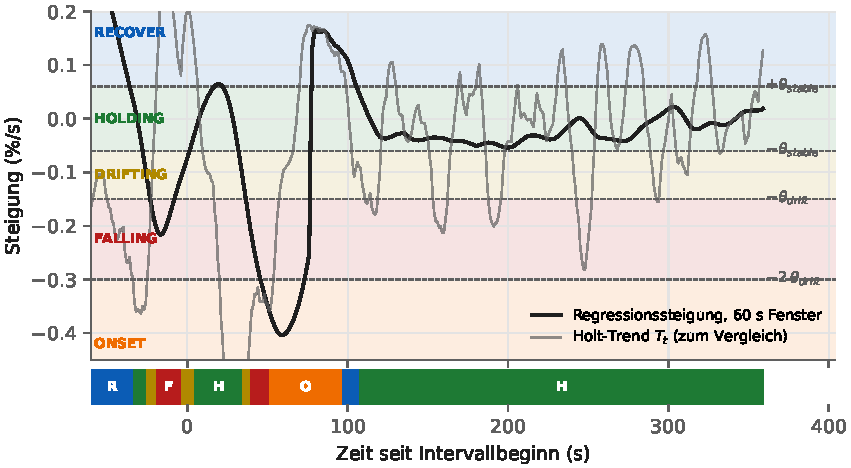
\includegraphics[width=\textwidth]{figures/slope.pdf}
  \caption{Regressionssteigung $s_t$ (schwarz) und Holt-Trend $T_t$ (grau)
    über dasselbe Intervall wie \cref{fig:signal}. Die Bänder sind die
    Zustandsklassen aus \cref{tab:states}. Während $s_t$ nach dem Transienten
    im Plateau-Band bleibt, pendelt $T_t$ durch drei Klassen. Der Zustand
    beschreibt die Mitte seines Fensters, deshalb läuft das Urteil der Form
    um etwa 30 Sekunden hinterher; die Ampel auf der Uhr trägt diese
    Verzögerung, die Einfärbung des Diagramms korrigiert sie durch ein auf
    jedes Segment zentriertes Fenster.}
  \label{fig:slope}
\end{figure}

% ---------------------------------------------------------------------------
\section{Zustandsklassifikation}

\subsection{Fünf Zustände}

Die Regressionssteigung wird in fünf Klassen eingeteilt (\cref{tab:states}).
Vier davon sind Aussagen über die Richtung der Sättigung; die fünfte, \ONSET{},
ist die Feststellung, dass noch kein Urteil möglich ist.

\begin{table}[H]
  \centering\small
  \caption{Zustände, Schwellen und Bedeutung. Die Steigungen gelten für die
    Standardwerte; in \permin{} multipliziert mit 60.}
  \label{tab:states}
  \begin{tabularx}{\textwidth}{@{}llX@{}}
    \toprule
    Zustand & Bedingung an $s_t$ (\pers) & Bedeutung \\
    \midrule
    \RECOVER  & $s_t > +\num{0.06}$ & Sättigung steigt: Erholung, oder die Belastung ist zu leicht \\
    \HOLDING  & $-\num{0.06} \le s_t \le +\num{0.06}$ & Plateau: Angebot deckt Verbrauch, nachhaltiger Steady State \\
    \DRIFTING & $-\num{0.15} \le s_t < -\num{0.06}$ & langsamer Abfall: fordernd, noch kontrolliert \\
    \FALLING  & $-\num{0.30} \le s_t < -\num{0.15}$ & der Abfall setzt sich fort: hier gibt es keinen Steady State \\
    \ONSET    & $s_t < -\num{0.30}$ & rapide Entsättigung: der On-Transient, kein Urteil \\
    \bottomrule
  \end{tabularx}
\end{table}

Die Namen benennen das gemessene Verhalten. Zonennummern fehlen absichtlich:
Eine Zone ist eine Aussage über die Intensität, während das Feld eine Steigung
misst, und ein Plateau tritt unterhalb der ersten Laktatschwelle ebenso auf
wie an der zweiten. Ohne die individuellen Oxygenierungs-Breakpoints des
Athleten kann keine Abbildung von Steigung auf Zone richtig sein.

Die Schwelle des On-Transienten ist an $\theta_{\mathrm{drift}}$ gekoppelt,
$\theta_{\mathrm{onkin}} = 2\,\theta_{\mathrm{drift}}$, damit sie beim
Abstimmen mitskaliert. Der Wert \num{0.30}~\pers{} liegt zwischen dem
Plateau-Extrem und der gemessenen Steilheit des Transienten.

\subsection{Hysterese}

Eine Steigung genau auf einer Grenze würde die Farbe flackern lassen. Deshalb
wird das Band, in dem sich das Feld gerade befindet, um den Faktor
$(1 \pm \eta)$ verbreitert, so dass ein Zustand schwerer zu verlassen als zu
halten ist. Mit $\eta = \num{0.15}$ gilt im Zustand \HOLDING{}
\begin{equation}
  \theta_{\mathrm{stable}}' = (1+\eta)\,\theta_{\mathrm{stable}} = \num{0.069}~\pers,
\end{equation}
im Zustand \DRIFTING{} entsprechend
$\theta_{\mathrm{stable}}' = (1-\eta)\,\theta_{\mathrm{stable}} = \num{0.051}$
und $\theta_{\mathrm{drift}}' = (1+\eta)\,\theta_{\mathrm{drift}} = \num{0.1725}$,
und so weiter für die übrigen Zustände. Eine Steigung von
\num{-0.065}~\pers{} ist damit \HOLDING{}, wenn das Feld bereits \HOLDING{}
zeigt, und \DRIFTING{}, wenn es aus \DRIFTING{} kommt.

\subsection{Verweildauer}

Zusätzlich muss ein neues Urteil $d = 3$ aufeinander folgende Updates lang
bestehen, bevor es angezeigt wird. Die Hysterese verbreitert das Band; die
Verweildauer fügt Zeit hinzu, und genau das fängt eine Steigung ab, die kurz
über eine Schwelle tritt und zurückkommt. Der Wert ist gemessen
(\cref{sec:robust}).

Die Verweildauer gilt nur für das \emph{angezeigte} Urteil. Die Logik des
On-Transienten (nächster Abschnitt) läuft auf der rohen Klassifikation mit
eigenem Zähler. Sie vom beruhigten Zustand zu treiben führt in eine
Verklemmung: Die Verweildauer hält \ONSET{} noch drei Schritte, nachdem der
Abfall geendet hat, diese Schritte spannen den Fensterneustart wieder, der
Neustart erzwingt \ONSET{}, und das Feld verlässt den Transienten nie. Der
Fehler ist bei der Entwicklung aufgetreten und wurde als 100~Prozent \ONSET{}
über jedes synthetische Intervall gemessen.

\subsection{Der On-Transient}
\label{sec:onset}

Jedes harte Intervall beginnt mit einem steilen Abfall, und der ist noch kein
Urteil über Nachhaltigkeit: Ein nachhaltiges und ein nicht nachhaltiges
Intervall beginnen gleich. Den Abfall selbst als \FALLING{} zu werten würde
jedes harte Intervall für seine erste Minute rot färben.

Deshalb bekommt der Transient einen eigenen Zustand, und wenn er endet, wird
das Regressionsfenster \emph{neu gestartet}. Die Plateau-Frage wird damit
ausschließlich aus Daten nach dem Transienten beantwortet. Konkret:
\begin{enumerate}
  \item Klassifiziert die rohe Steigung $d$ Schritte in Folge als \ONSET{}, gilt
        ein Transient als im Gang. Die steilste Steigung wird als
        On-Kinetik-Rate des Intervalls festgehalten.
  \item Verlässt die rohe Steigung das \ONSET{}-Band, wird das Fenster geleert
        und mit dem aktuellen Level neu begonnen. Bis es zu einem Drittel
        gefüllt ist, meldet das Feld weiter \ONSET{}.
  \item Ein Lap-Druck gilt ebenfalls als Lastwechsel und startet das Fenster
        neu, weil der alte Fit eine Last beschreibt, die nicht mehr anliegt.
\end{enumerate}

Die Bedeutung liegt in der Folge der Zustände, nicht im Abfall: \ONSET{}, dann
\HOLDING{} ist eine nachhaltige Belastung; \ONSET{}, dann \DRIFTING{} oder
\FALLING{} ohne Plateau ist eine Belastung oberhalb des Punktes, an dem ein
Steady State existiert. \Cref{fig:synthetic} zeigt beide Fälle an
synthetischen Daten mit bekannter Wahrheit.

\begin{figure}[H]
  \centering
  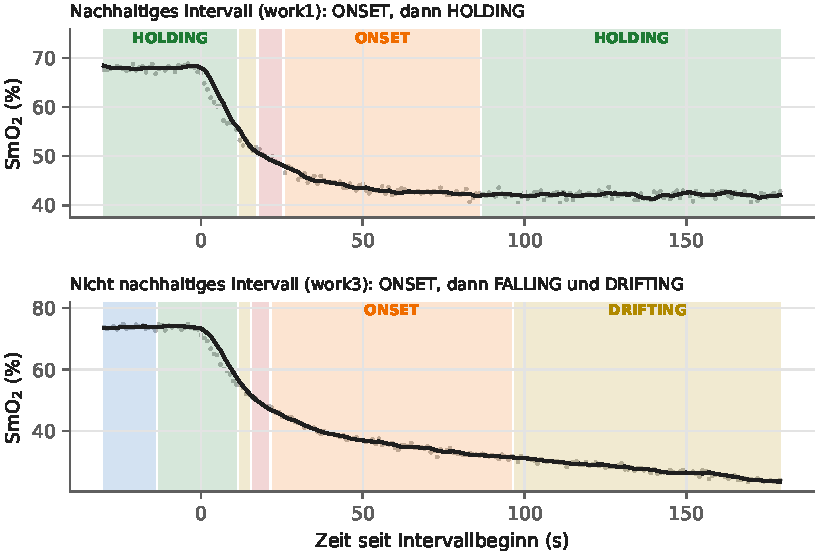
\includegraphics[width=\textwidth]{figures/synthetic.pdf}
  \caption{Synthetische Intervalle mit bekannter Wahrheit. Oben ein
    nachhaltiges Intervall: nach dem Transienten \SI{\nSynOneSteady}{\percent}
    der Zeit \HOLDING{}. Unten ein nicht nachhaltiges: \SI{\nSynThreeSteady}{\percent}
    \HOLDING{}, der Rest Abfall und Drift. Synthetische Daten dienen nur der
    Regressionskontrolle; die Schwellen sind an echten Einheiten gemessen,
    weil ein früherer, zu sauberer Generator Schwellen lieferte, die um eine
    Größenordnung zu eng waren.}
  \label{fig:synthetic}
\end{figure}

\paragraph{Abgrenzung gegen echtes Absinken oberhalb der Schwelle.}
Eine Belastung über der zweiten Laktatschwelle senkt die Sättigung ebenfalls.
Drei Dinge verhindern, dass das Feld sie dauerhaft als Transient abtut. Erstens
die Steilheit: Ein On-Transient unterschreitet gemessen \num{-0.23}~\pers, ein
Absinken oberhalb der Schwelle liegt nach der ersten Minute im Bereich von
\num{0.06} bis \num{0.30}~\pers, den \DRIFTING{} und \FALLING{} abdecken.
Zweitens hat das Signal einen Boden: Ein Abfall von \num{0.30}~\pers{} über
drei Minuten wären 54 Prozentpunkte, so viel Spanne hat kein Sensor, die Kurve
muss verflachen und verlässt das \ONSET{}-Band. Drittens die Reihenfolge, wie
oben beschrieben. Schlecht behandelt wird ein Fall: eine sehr harte Belastung
aus bereits niedriger Sättigung, wo der Abfall nur flach ist, weil nach unten
kein Platz mehr ist. Das Feld nennt es ein Plateau, und nur das Minimum und
die Skala des Diagramms zeigen, dass es ein Plateau am Boden der Spanne ist.

% ---------------------------------------------------------------------------
\section{Robustheit gegen Ausreißer}
\label{sec:robust}

Drei Maßnahmen sitzen an drei Stellen außerhalb der Klassifikation, damit die
Schwellen ihre gemessene Bedeutung behalten: der Median aus
\cref{sec:two-timescales}, eine Toleranz für kurze Datenlöcher, und die
Verweildauer.

Ein einzelner ungültiger Messwert löschte in einer früheren Version das ganze
Regressionsfenster, was das Fenster plus seine 20~Sekunden Wiederauffüllung
kostete: rund 80 Sekunden \enquote{noch nicht entschieden} für eine schlechte
Sekunde. Das Fenster führt pro Messwert einen Zeitstempel und skaliert die
Steigung nach \cref{eq:slope} über die echte Zeitspanne, ein Loch von wenigen
Sekunden kostet also Genauigkeit und nicht Gültigkeit. Fit und letztes Urteil
werden jetzt bis zu 8 Sekunden gehalten.

Die Verweildauer ist an der Referenzeinheit gemessen. Zählt man Zustandsphasen
unter 5 Sekunden als Flackern, ergibt sich \cref{tab:dwell}. Vier wäre noch
ruhiger und wird nicht genommen: Jeder Wiedereintritt in einen Zustand zahlt
die Verweildauer erneut, und eine kurze Erholungsrunde hat wenige Sekunden
übrig. In einer der Vergleichseinheiten fiel eine 59 Sekunden lange
Erholungsrunde bei $d = 4$ von 72 auf 50 Prozent \RECOVER{}, genau auf die
dokumentierte Untergrenze. Drei halbiert das Flackern für wenige Punkte.

\begin{table}[H]
  \centering\small
  \caption{Flackern in Abhängigkeit von der Verweildauer, Referenzeinheit.}
  \label{tab:dwell}
  \begin{tabular}{@{}ccc@{}}
    \toprule
    Verweildauer $d$ & Zustandsphasen gesamt & davon kürzer als \SI{5}{\second} \\
    \midrule
    1 (keine) & \nRunsOne   & \nDwellOne \\
    2         & \nRunsTwo   & \nDwellTwo \\
    \textbf{3 (Standard)} & \textbf{\nRunsThree} & \textbf{\nDwellThree} \\
    4         & \nRunsFour  & \nDwellFour \\
    \bottomrule
  \end{tabular}
\end{table}

% ---------------------------------------------------------------------------
\section{Metriken}

\subsection{Änderungsrate}

Die angezeigte Rate ist die Regressionssteigung $s_t$, dieselbe Größe, aus der
die Farbe bestimmt wird. Eine Zahl, die der Farbe widerspräche, würde nur
verwirren. Die Einheit ist wählbar: \pers{} ist die natürliche Einheit der
Regression, aber am Plateau steht dort \num{-0.01} und jede interessante Stelle
liegt hinter dem Komma; \permin{} hebt die Zahlen in einen Bereich, den man auf
einen Blick vergleichen kann. Beim Standardwert $\theta_{\mathrm{stable}} =
\num{0.06}$~\pers{} entspricht die Plateau-Grenze \num{3.6}~\permin: Ein
vierminütiges Intervall darf 14 Punkte verlieren und gilt an der Grenze noch
als flach. Das ist die ehrliche Lesart der Einstellung.

\subsection{Rundenstatistik und Control Index}
\label{sec:sci}

Beim Lap-Druck werden für das abgeschlossene Intervall mit Startwert $L_0$,
Endwert $L_1$ und Dauer $D$ geschrieben:
\begin{align}
  \text{Desaturationsrate} &= \frac{L_1 - L_0}{D} && (\pers) \\
  \text{SCI}_{\mathrm{drop}} &= L_0 - L_1 && \text{(Prozentpunkte)} \label{eq:sci-drop}\\
  \text{SCI}_{\mathrm{ratio}} &= \frac{L_1}{L_0} && \text{(dimensionslos)} \label{eq:sci-ratio}
\end{align}
dazu Minimum, Maximum und die steilste Steigung des On-Transienten
(On-Kinetik-Rate), die mit der metabolischen Rate korreliert.

Der \emph{SmO\textsubscript{2} Control Index} ist die Amplitude der
Entsättigung eines Intervalls: wie weit die Belastung die Sättigung von dem
Niveau heruntergezogen hat, auf dem sie begonnen hat. Im Stufentest korreliert
diese Amplitude mit dem Laktat, und sie ist genau das, was die
Desaturationsrate wegwirft: Das Teilen durch die Dauer macht die Rate zwischen
Stufen verschiedener Länge vergleichbar, und die Amplitude ist der Teil, den
das Teilen entfernt. Der Index hängt daher an der Stufenlänge, und das ist
eine Eigenschaft der Messung: Stufen gleicher Länge vergleichen. Beide Formen
werden geschrieben, weil offen ist, welche zwischen Stufenlängen besser trägt.

Live zeigt das Feld dieselben Größen gegen den Startwert der \emph{aktuellen}
Runde; sie zählen mit dem Intervall hoch und landen beim Lap-Druck auf dem
aufgezeichneten Wert.

\paragraph{Beispielrechnung.}
Das Intervall aus \cref{fig:signal}: $L_0 = \SI{\nSciStart}{\percent}$,
$L_1 = \SI{\nSciEnd}{\percent}$, $D = \SI{\nSciDur}{\second}$.
\begin{equation*}
  \text{Rate} = \frac{\num{\nSciEnd} - \num{\nSciStart}}{\num{\nSciDur}} = \num{\nSciRate}~\pers, \quad
  \text{SCI}_{\mathrm{drop}} = \num{\nSciStart} - \num{\nSciEnd} = \num{\nSciDrop}, \quad
  \text{SCI}_{\mathrm{ratio}} = \frac{\num{\nSciEnd}}{\num{\nSciStart}} = \num{\nSciRatio}.
\end{equation*}

\paragraph{Stufentest.}
Die Referenzeinheit enthält sechs Arbeitsstufen gleicher Länge.
\Cref{tab:steps} und \cref{fig:sci} zeigen, wie sich der Index über die
Stufen entwickelt: monoton bis zur letzten Stufe, in beiden Formen. Die
Desaturationsrate trägt dieselbe Information schwächer, weil die Stufen gleich
lang sind und der Nenner nichts unterscheidet.

\begin{table}[H]
  \centering\small
  \caption{Arbeitsstufen der Referenzeinheit. Start und Ende in \si{\percent},
    Abfall in Prozentpunkten, Rate in \pers, HOLDING als Anteil der Stufenzeit.}
  \label{tab:steps}
  \begin{tabular}{@{}cccccccc@{}}
    \toprule
    Stufe & Dauer (s) & Start & Ende & SCI$_{\mathrm{drop}}$ & SCI$_{\mathrm{ratio}}$ & Rate & HOLDING (\si{\percent}) \\
    \midrule
    \nStepsRows
    \bottomrule
  \end{tabular}
\end{table}

\begin{figure}[H]
  \centering
  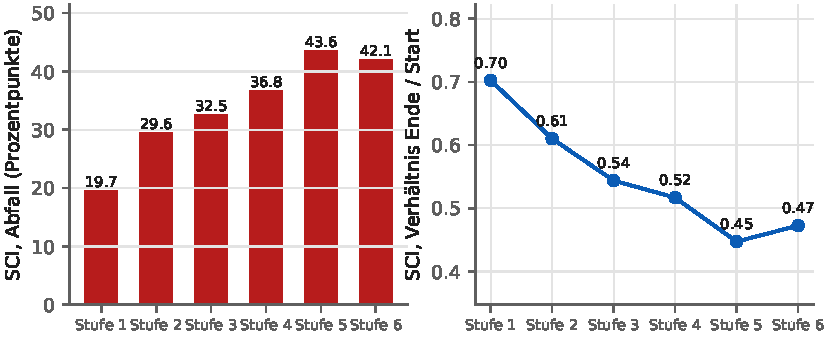
\includegraphics[width=\textwidth]{figures/sci.pdf}
  \caption{Der Control Index über die sechs Arbeitsstufen, links als Abfall in
    Prozentpunkten, rechts als Verhältnis Ende zu Start. Beide steigen
    beziehungsweise fallen monoton bis zur letzten Stufe; die letzte liegt
    innerhalb der Schwankung der vorletzten.}
  \label{fig:sci}
\end{figure}

\subsection{Spanne und Mittelwert}

Minimum und Maximum der Einheit werden aus dem geglätteten Level
fortgeschrieben, nie aus Rohwerten, und relaxieren mit \num{0.02}~\pers{} zum
aktuellen Wert zurück, sobald sie mehr als 3 Punkte von ihm entfernt sind, so
dass ein Ausreißer die Skala nicht für den Rest der Einheit definiert. Sie
bilden die Zellen MIN und MAX und die Y-Achse des Diagramms; die Runde hat
eigene Extrema ohne Relaxation. Der Mittelwert läuft nur bei laufendem Timer
und existiert je Einheit und je Runde.

\subsection{Entkopplung}

Das Feld beobachtet die externe Last, Leistung auf dem Rad oder Geschwindigkeit
beziehungsweise Pace, über ein Fenster von 30 Sekunden. Ist deren
Variationskoeffizient
\begin{equation}
  c_v = \frac{\sigma_{\mathrm{Last}}}{\mu_{\mathrm{Last}}} < \num{0.04}
\end{equation}
und der Zustand gleichzeitig \DRIFTING{} oder \FALLING{}, wird Entkopplung
gemeldet: Bei konstanter äußerer Last sinkt die Oxygenierung weiter. Das ist
beginnende Ermüdung oder Effizienzverlust, und es ist in keinem der beiden
Signale allein sichtbar.

% ---------------------------------------------------------------------------
\section{Prognose}
\label{sec:forecast}

Aus Level und Holt-Trend folgt eine lineare Extrapolation über den Horizont $h$:
\begin{equation}
  \hat L_{t+h} = L_t + T_t \, h, \qquad 0 \le \hat L_{t+h} \le 100.
  \label{eq:forecast}
\end{equation}
Das Diagramm zeigt sie als Nadel am rechten Rand, die auf die Höhe zeigt, auf
die der Trend zuläuft.

\paragraph{Beispielrechnung.}
\SI{\nFcT}{\second} nach Beginn von \nFcLap{}: $L_t = \num{\nFcLevel}$,
$T_t = \num{\nFcTrend}$~\pers, $h = \SI{15}{\second}$.
\begin{equation*}
  \hat L_{t+15} = \num{\nFcLevel} + (\num{\nFcTrend}) \cdot 15 = \num{\nFcPred}~\si{\percent}.
\end{equation*}
15 Sekunden später betrug der Level tatsächlich \SI{\nFcActual}{\percent}, der
Fehler also \num{\nFcErr} Punkte.

\paragraph{Bewertung.}
Ein einzelnes Beispiel sagt wenig; deshalb wurde die Prognose über die gesamte
Einheit gegen den realisierten Level 15~Sekunden später verglichen, getrennt
nach dem Zustand im Moment der Prognose (\cref{tab:forecast}). Als Referenz
dient die naive Annahme, der Wert bleibe, wo er ist: $\hat L_{t+h} = L_t$.

\begin{table}[H]
  \centering\small
  \caption{Wurzel des mittleren quadratischen Prognosefehlers (RMSE) über
    15~Sekunden, Referenzeinheit, in Prozentpunkten.}
  \label{tab:forecast}
  \begin{tabular}{@{}lc@{}}
    \toprule
    Prognose & RMSE \\
    \midrule
    Holt, $L_t + T_t h$, alle Zustände & \num{\nFcRmseAll} \\
    \quad davon im Zustand \HOLDING{}  & \num{\nFcRmseHolding} \\
    \quad davon im Zustand \DRIFTING{} & \num{\nFcRmseDrifting} \\
    \quad davon im Zustand \FALLING{}  & \num{\nFcRmseFalling} \\
    \quad davon im Zustand \RECOVER{}  & \num{\nFcRmseRecover} \\
    \quad davon im Zustand \ONSET{}    & \num{\nFcRmseOnset} \\
    \midrule
    Naiv, $L_t$ (der Wert bleibt) & \num{\nFcRmseNaive} \\
    \bottomrule
  \end{tabular}
\end{table}

Das Ergebnis fällt gegen das Modell aus und gehört deshalb hierher: Auf dieser
Einheit ist die Holt-Extrapolation über 15~Sekunden mit \num{\nFcRmseAll}
Punkten \emph{schlechter} als die naive Annahme mit \num{\nFcRmseNaive}. Der
Grund ist in \cref{fig:forecast} sichtbar. Der Trend $T_t$ ist die schnelle
Größe, die in \cref{sec:two-timescales} als zu unruhig für die Klassifikation
befunden wurde, und dieselbe Unruhe mit 15 multipliziert überschießt an jeder
Biegung der Kurve. Im Plateau, wo der Trend klein ist, ist der Fehler am
kleinsten; im Transienten, wo er groß ist, am größten.

\begin{figure}[tbp]
  \centering
  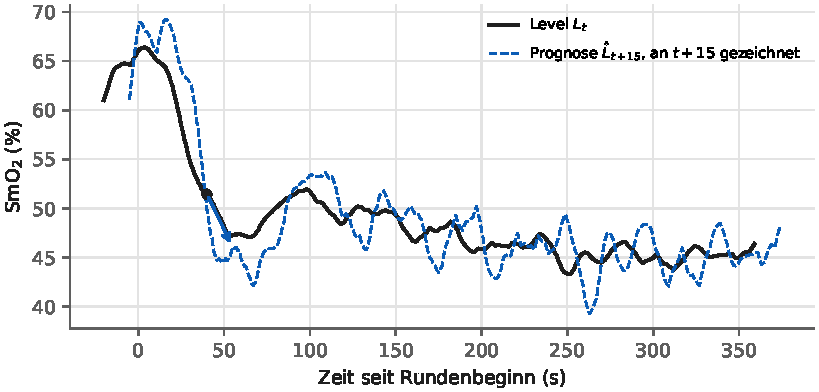
\includegraphics[width=\textwidth]{figures/forecast.pdf}
  \caption{Level $L_t$ und die 15-Sekunden-Prognose, jeweils an dem Zeitpunkt
    gezeichnet, über den sie eine Aussage macht. Der Pfeil ist die
    Beispielrechnung. Die Prognose überschießt an jeder Biegung, weil sie die
    momentane Steigung geradlinig fortsetzt.}
  \label{fig:forecast}
\end{figure}

Für die Nutzung folgt daraus: Die Nadel ist ein \emph{Richtungsanzeiger}, kein
Prädiktor. Sie sagt verlässlich, wohin sich der Wert gerade bewegt, und
unzuverlässig, wo er ankommt. Wer eine Zahl braucht, ist mit dem Level und dem
Zustand besser bedient. Für eine bessere Prognose wären ein kleineres $\beta$,
ein kürzerer Horizont oder eine Extrapolation der Regressionssteigung statt des
Holt-Trends die naheliegenden Kandidaten; keiner davon ist bisher gegen Daten
geprüft.

% ---------------------------------------------------------------------------
\section{Grenzen}

\begin{itemize}
  \item Das Feld misst eine Steigung und keine Intensität. Ein Plateau auf
        niedrigem Niveau und ein Plateau auf hohem Niveau sind ihm gleich; die
        Einordnung in Intensitätsbereiche braucht die individuellen
        Oxygenierungs-Breakpoints, die ein Datenfeld nicht messen kann.
  \item Der Zustand beschreibt die Mitte seines Fensters und läuft der Form der
        Kurve um etwa 30 Sekunden plus Verweildauer hinterher.
  \item Der Control Index hängt an der Stufenlänge. Er ist zwischen Stufen
        gleicher Länge vergleichbar und sonst nicht.
  \item Die Prognose ist auf der Referenzeinheit nicht besser als Persistenz
        (\cref{sec:forecast}).
  \item Die Schwellen sind an fünf Einheiten einer Person gemessen. Sie sind
        einstellbar, und das Werkzeug \texttt{tools/kinetics\_replay.py}
        rechnet dasselbe Modell über eigene Aufzeichnungen, damit die
        Abstimmung gegen bekannte Intervalle erfolgt und nicht gegen ein
        Gefühl.
\end{itemize}

\appendix
\section{Reproduzierbarkeit}

Alle Abbildungen und alle Zahlen dieses Dokuments erzeugt
\texttt{docs/paper/figures.py} aus einer FIT-Datei, indem es die
Python-Portierung des Uhrenmodells (\texttt{tools/kinetics\_replay.py}) über
die Aufzeichnung laufen lässt. Die Zahlen werden als LaTeX-Makros nach
\texttt{numbers.tex} geschrieben und hier eingebunden; im Text steht keine
einzige von Hand eingetragene Messzahl. Eine andere Datei ergibt ein Dokument
mit deren Zahlen.

\end{document}
